\documentclass[1p]{elsarticle_modified}
%\bibliographystyle{elsarticle-num}

%\usepackage[colorlinks]{hyperref}
%\usepackage{abbrmath_seonhwa} %\Abb, \Ascr, \Acal ,\Abf, \Afrak
\usepackage{amsfonts}
\usepackage{amssymb}
\usepackage{amsmath}
\usepackage{amsthm}
\usepackage{scalefnt}
\usepackage{amsbsy}
\usepackage{kotex}
\usepackage{caption}
\usepackage{subfig}
\usepackage{color}
\usepackage{graphicx}
\usepackage{xcolor} %% white, black, red, green, blue, cyan, magenta, yellow
\usepackage{float}
\usepackage{setspace}
\usepackage{hyperref}

\usepackage{tikz}
\usetikzlibrary{arrows}

\usepackage{multirow}
\usepackage{array} % fixed length table
\usepackage{hhline}

%%%%%%%%%%%%%%%%%%%%%
\makeatletter
\renewcommand*\env@matrix[1][\arraystretch]{%
	\edef\arraystretch{#1}%
	\hskip -\arraycolsep
	\let\@ifnextchar\new@ifnextchar
	\array{*\c@MaxMatrixCols c}}
\makeatother %https://tex.stackexchange.com/questions/14071/how-can-i-increase-the-line-spacing-in-a-matrix
%%%%%%%%%%%%%%%

\usepackage[normalem]{ulem}

\newcommand{\msout}[1]{\ifmmode\text{\sout{\ensuremath{#1}}}\else\sout{#1}\fi}
%SOURCE: \msout is \stkout macro in https://tex.stackexchange.com/questions/20609/strikeout-in-math-mode

\newcommand{\cancel}[1]{
	\ifmmode
	{\color{red}\msout{#1}}
	\else
	{\color{red}\sout{#1}}
	\fi
}

\newcommand{\add}[1]{
	{\color{blue}\uwave{#1}}
}

\newcommand{\replace}[2]{
	\ifmmode
	{\color{red}\msout{#1}}{\color{blue}\uwave{#2}}
	\else
	{\color{red}\sout{#1}}{\color{blue}\uwave{#2}}
	\fi
}

\newcommand{\Sol}{\mathcal{S}} %segment
\newcommand{\D}{D} %diagram
\newcommand{\A}{\mathcal{A}} %arc


%%%%%%%%%%%%%%%%%%%%%%%%%%%%%5 test

\def\sl{\operatorname{\textup{SL}}(2,\Cbb)}
\def\psl{\operatorname{\textup{PSL}}(2,\Cbb)}
\def\quan{\mkern 1mu \triangleright \mkern 1mu}

\theoremstyle{definition}
\newtheorem{thm}{Theorem}[section]
\newtheorem{prop}[thm]{Proposition}
\newtheorem{lem}[thm]{Lemma}
\newtheorem{ques}[thm]{Question}
\newtheorem{cor}[thm]{Corollary}
\newtheorem{defn}[thm]{Definition}
\newtheorem{exam}[thm]{Example}
\newtheorem{rmk}[thm]{Remark}
\newtheorem{alg}[thm]{Algorithm}

\newcommand{\I}{\sqrt{-1}}
\begin{document}

%\begin{frontmatter}
%
%\title{Boundary parabolic representations of knots up to 8 crossings}
%
%%% Group authors per affiliation:
%\author{Yunhi Cho} 
%\address{Department of Mathematics, University of Seoul, Seoul, Korea}
%\ead{yhcho@uos.ac.kr}
%
%
%\author{Seonhwa Kim} %\fnref{s_kim}}
%\address{Center for Geometry and Physics, Institute for Basic Science, Pohang, 37673, Korea}
%\ead{ryeona17@ibs.re.kr}
%
%\author{Hyuk Kim}
%\address{Department of Mathematical Sciences, Seoul National University, Seoul 08826, Korea}
%\ead{hyukkim@snu.ac.kr}
%
%\author{Seokbeom Yoon}
%\address{Department of Mathematical Sciences, Seoul National University, Seoul, 08826,  Korea}
%\ead{sbyoon15@snu.ac.kr}
%
%\begin{abstract}
%We find all boundary parabolic representation of knots up to 8 crossings.
%
%\end{abstract}
%\begin{keyword}
%    \MSC[2010] 57M25 
%\end{keyword}
%
%\end{frontmatter}

%\linenumbers
%\tableofcontents
%
\newcommand\colored[1]{\textcolor{white}{\rule[-0.35ex]{0.8em}{1.4ex}}\kern-0.8em\color{red} #1}%
%\newcommand\colored[1]{\textcolor{white}{ #1}\kern-2.17ex	\textcolor{white}{ #1}\kern-1.81ex	\textcolor{white}{ #1}\kern-2.15ex\color{red}#1	}

{\Large $\underline{11a_{49}~(K11a_{49})}$}

\setlength{\tabcolsep}{10pt}
\renewcommand{\arraystretch}{1.6}
\vspace{1cm}\begin{tabular}{m{100pt}>{\centering\arraybackslash}m{274pt}}
\multirow{5}{120pt}{
	\centering
	\includegraphics[width=112pt]{../../../GIT/diagram.site/Diagrams/png/298_11a_49.png}\\
\ \ \ A knot diagram\footnotemark}&
\allowdisplaybreaks
\textbf{Linearized knot diagam} \\
\cline{2-2}
 &
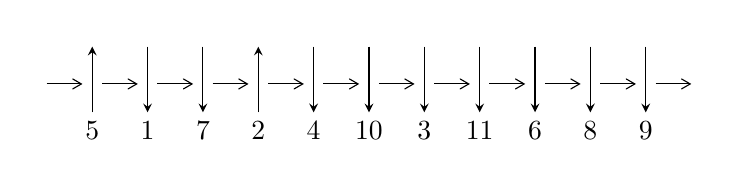
\begin{tikzpicture}[x=20pt, y=17pt]
	% nodes
	\node (C0) at (0, 0) {};
	\node (C1) at (1, 0) {};
	\node (C1U) at (1, +1) {};
	\node (C1D) at (1, -1) {5};

	\node (C2) at (2, 0) {};
	\node (C2U) at (2, +1) {};
	\node (C2D) at (2, -1) {1};

	\node (C3) at (3, 0) {};
	\node (C3U) at (3, +1) {};
	\node (C3D) at (3, -1) {7};

	\node (C4) at (4, 0) {};
	\node (C4U) at (4, +1) {};
	\node (C4D) at (4, -1) {2};

	\node (C5) at (5, 0) {};
	\node (C5U) at (5, +1) {};
	\node (C5D) at (5, -1) {4};

	\node (C6) at (6, 0) {};
	\node (C6U) at (6, +1) {};
	\node (C6D) at (6, -1) {10};

	\node (C7) at (7, 0) {};
	\node (C7U) at (7, +1) {};
	\node (C7D) at (7, -1) {3};

	\node (C8) at (8, 0) {};
	\node (C8U) at (8, +1) {};
	\node (C8D) at (8, -1) {11};

	\node (C9) at (9, 0) {};
	\node (C9U) at (9, +1) {};
	\node (C9D) at (9, -1) {6};

	\node (C10) at (10, 0) {};
	\node (C10U) at (10, +1) {};
	\node (C10D) at (10, -1) {8};

	\node (C11) at (11, 0) {};
	\node (C11U) at (11, +1) {};
	\node (C11D) at (11, -1) {9};
	\node (C12) at (12, 0) {};

	% arrows
	\draw[->,>={angle 60}]
	(C0) edge (C1) (C1) edge (C2) (C2) edge (C3) (C3) edge (C4) (C4) edge (C5) (C5) edge (C6) (C6) edge (C7) (C7) edge (C8) (C8) edge (C9) (C9) edge (C10) (C10) edge (C11) (C11) edge (C12) ;	\draw[->,>=stealth]
	(C1D) edge (C1U) (C2U) edge (C2D) (C3U) edge (C3D) (C4D) edge (C4U) (C5U) edge (C5D) (C6U) edge (C6D) (C7U) edge (C7D) (C8U) edge (C8D) (C9U) edge (C9D) (C10U) edge (C10D) (C11U) edge (C11D) ;
	\end{tikzpicture} \\
\hhline{~~} \\& 
\textbf{Solving Sequence} \\ \cline{2-2} 
 &
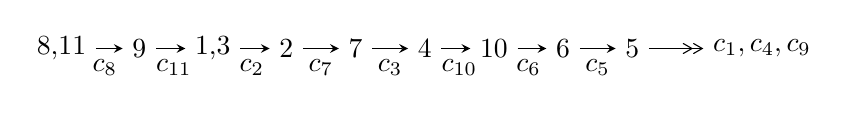
\begin{tikzpicture}[x=25pt, y=7pt]
	% node
	\node (A0) at (-1/8, 0) {8,11};
	\node (A1) at (1, 0) {9};
	\node (A2) at (33/16, 0) {1,3};
	\node (A3) at (25/8, 0) {2};
	\node (A4) at (33/8, 0) {7};
	\node (A5) at (41/8, 0) {4};
	\node (A6) at (49/8, 0) {10};
	\node (A7) at (57/8, 0) {6};
	\node (A8) at (65/8, 0) {5};
	\node (C1) at (1/2, -1) {$c_{8}$};
	\node (C2) at (3/2, -1) {$c_{11}$};
	\node (C3) at (21/8, -1) {$c_{2}$};
	\node (C4) at (29/8, -1) {$c_{7}$};
	\node (C5) at (37/8, -1) {$c_{3}$};
	\node (C6) at (45/8, -1) {$c_{10}$};
	\node (C7) at (53/8, -1) {$c_{6}$};
	\node (C8) at (61/8, -1) {$c_{5}$};
	\node (A9) at (10, 0) {$c_{1},c_{4},c_{9}$};

	% edge
	\draw[->,>=stealth]	
	(A0) edge (A1) (A1) edge (A2) (A2) edge (A3) (A3) edge (A4) (A4) edge (A5) (A5) edge (A6) (A6) edge (A7) (A7) edge (A8) ;
	\draw[->>,>={angle 60}]	
	(A8) edge (A9);
\end{tikzpicture} \\ 

\end{tabular} \\

\footnotetext{
The image of knot diagram is generated by the software ``\textbf{Draw programme}" developed by Andrew Bartholomew(\url{http://www.layer8.co.uk/maths/draw/index.htm\#Running-draw}), where we modified some parts for our purpose(\url{https://github.com/CATsTAILs/LinksPainter}).
}\phantom \\ \newline 
\centering \textbf{Ideals for irreducible components\footnotemark of $X_{\text{par}}$} 
 
\begin{align*}
I^u_{1}&=\langle 
9.01751\times10^{36} u^{59}+5.15573\times10^{37} u^{58}+\cdots+2.98614\times10^{35} b-6.79357\times10^{36},\\
\phantom{I^u_{1}}&\phantom{= \langle  }8.91336\times10^{36} u^{59}+4.98175\times10^{37} u^{58}+\cdots+2.98614\times10^{35} a-5.40121\times10^{36},\;u^{60}+7 u^{59}+\cdots-6 u-1\rangle \\
I^u_{2}&=\langle 
- a^2+b-2 a-1,\;a^4+3 a^3+4 a^2+3 a+2,\;u-1\rangle \\
I^u_{3}&=\langle 
b,\;a^2+a u+2 a+3 u+5,\;u^2+u-1\rangle \\
\\
\end{align*}
\raggedright * 3 irreducible components of $\dim_{\mathbb{C}}=0$, with total 68 representations.\\
\footnotetext{All coefficients of polynomials are rational numbers. But the coefficients are sometimes approximated in decimal forms when there is not enough margin.}
\newpage
\renewcommand{\arraystretch}{1}
\centering \section*{I. $I^u_{1}= \langle 9.02\times10^{36} u^{59}+5.16\times10^{37} u^{58}+\cdots+2.99\times10^{35} b-6.79\times10^{36},\;8.91\times10^{36} u^{59}+4.98\times10^{37} u^{58}+\cdots+2.99\times10^{35} a-5.40\times10^{36},\;u^{60}+7 u^{59}+\cdots-6 u-1 \rangle$}
\flushleft \textbf{(i) Arc colorings}\\
\begin{tabular}{m{7pt} m{180pt} m{7pt} m{180pt} }
\flushright $a_{8}=$&$\begin{pmatrix}1\\0\end{pmatrix}$ \\
\flushright $a_{11}=$&$\begin{pmatrix}0\\u\end{pmatrix}$ \\
\flushright $a_{9}=$&$\begin{pmatrix}1\\u^2\end{pmatrix}$ \\
\flushright $a_{1}=$&$\begin{pmatrix}- u\\- u^3+u\end{pmatrix}$ \\
\flushright $a_{3}=$&$\begin{pmatrix}-29.8491 u^{59}-166.829 u^{58}+\cdots+129.411 u+18.0876\\-30.1979 u^{59}-172.655 u^{58}+\cdots+122.504 u+22.7504\end{pmatrix}$ \\
\flushright $a_{2}=$&$\begin{pmatrix}-38.7260 u^{59}-215.837 u^{58}+\cdots+161.430 u+23.9641\\-40.2858 u^{59}-229.747 u^{58}+\cdots+160.391 u+30.0045\end{pmatrix}$ \\
\flushright $a_{7}=$&$\begin{pmatrix}-35.9915 u^{59}-204.169 u^{58}+\cdots+147.701 u+26.5908\\-36.2977 u^{59}-209.779 u^{58}+\cdots+151.862 u+29.1133\end{pmatrix}$ \\
\flushright $a_{4}=$&$\begin{pmatrix}-37.1833 u^{59}-206.920 u^{58}+\cdots+154.103 u+23.9174\\-41.6797 u^{59}-236.581 u^{58}+\cdots+163.204 u+30.6805\end{pmatrix}$ \\
\flushright $a_{10}=$&$\begin{pmatrix}u\\u\end{pmatrix}$ \\
\flushright $a_{6}=$&$\begin{pmatrix}-25.6472 u^{59}-153.577 u^{58}+\cdots+126.598 u+23.1246\\-25.9534 u^{59}-159.186 u^{58}+\cdots+130.758 u+25.6472\end{pmatrix}$ \\
\flushright $a_{5}=$&$\begin{pmatrix}-23.4754 u^{59}-130.115 u^{58}+\cdots+100.960 u+15.9285\\-27.6129 u^{59}-156.128 u^{58}+\cdots+107.032 u+20.4621\end{pmatrix}$\\ \flushright $a_{5}=$&$\begin{pmatrix}-23.4754 u^{59}-130.115 u^{58}+\cdots+100.960 u+15.9285\\-27.6129 u^{59}-156.128 u^{58}+\cdots+107.032 u+20.4621\end{pmatrix}$\\&\end{tabular}
\flushleft \textbf{(ii) Obstruction class $= -1$}\\~\\
\flushleft \textbf{(iii) Cusp Shapes $= 50.7022 u^{59}+278.914 u^{58}+\cdots-202.739 u-39.8944$}\\~\\
\newpage\renewcommand{\arraystretch}{1}
\flushleft \textbf{(iv) u-Polynomials at the component}\newline \\
\begin{tabular}{m{50pt}|m{274pt}}
Crossings & \hspace{64pt}u-Polynomials at each crossing \\
\hline $$\begin{aligned}c_{1},c_{4}\end{aligned}$$&$\begin{aligned}
&u^{60}+4 u^{59}+\cdots+6 u+1
\end{aligned}$\\
\hline $$\begin{aligned}c_{2},c_{5}\end{aligned}$$&$\begin{aligned}
&u^{60}+20 u^{59}+\cdots-82 u+1
\end{aligned}$\\
\hline $$\begin{aligned}c_{3},c_{7}\end{aligned}$$&$\begin{aligned}
&u^{60}-2 u^{59}+\cdots-16 u+16
\end{aligned}$\\
\hline $$\begin{aligned}c_{6},c_{9}\end{aligned}$$&$\begin{aligned}
&u^{60}+3 u^{59}+\cdots-24 u-16
\end{aligned}$\\
\hline $$\begin{aligned}c_{8},c_{10},c_{11}\end{aligned}$$&$\begin{aligned}
&u^{60}-7 u^{59}+\cdots+6 u-1
\end{aligned}$\\
\hline
\end{tabular}\\~\\
\newpage\renewcommand{\arraystretch}{1}
\flushleft \textbf{(v) Riley Polynomials at the component}\newline \\
\begin{tabular}{m{50pt}|m{274pt}}
Crossings & \hspace{64pt}Riley Polynomials at each crossing \\
\hline $$\begin{aligned}c_{1},c_{4}\end{aligned}$$&$\begin{aligned}
&y^{60}+20 y^{59}+\cdots-82 y+1
\end{aligned}$\\
\hline $$\begin{aligned}c_{2},c_{5}\end{aligned}$$&$\begin{aligned}
&y^{60}+44 y^{59}+\cdots-7010 y+1
\end{aligned}$\\
\hline $$\begin{aligned}c_{3},c_{7}\end{aligned}$$&$\begin{aligned}
&y^{60}+30 y^{59}+\cdots+1408 y+256
\end{aligned}$\\
\hline $$\begin{aligned}c_{6},c_{9}\end{aligned}$$&$\begin{aligned}
&y^{60}-33 y^{59}+\cdots-576 y+256
\end{aligned}$\\
\hline $$\begin{aligned}c_{8},c_{10},c_{11}\end{aligned}$$&$\begin{aligned}
&y^{60}-57 y^{59}+\cdots-48 y+1
\end{aligned}$\\
\hline
\end{tabular}\\~\\
\newpage\flushleft \textbf{(vi) Complex Volumes and Cusp Shapes}
$$\begin{array}{c|c|c}  
\text{Solutions to }I^u_{1}& \I (\text{vol} + \sqrt{-1}CS) & \text{Cusp shape}\\
 \hline 
\begin{aligned}
u &= \phantom{-}0.318501 + 0.946527 I \\
a &= \phantom{-}0.673424 - 0.443134 I \\
b &= \phantom{-}0.628475 + 1.190740 I\end{aligned}
 & \phantom{-}3.14485 - 10.38850 I & \phantom{-0.000000 } 0 \\ \hline\begin{aligned}
u &= \phantom{-}0.318501 - 0.946527 I \\
a &= \phantom{-}0.673424 + 0.443134 I \\
b &= \phantom{-}0.628475 - 1.190740 I\end{aligned}
 & \phantom{-}3.14485 + 10.38850 I & \phantom{-0.000000 } 0 \\ \hline\begin{aligned}
u &= \phantom{-}0.260347 + 0.914658 I \\
a &= -0.502988 + 0.479081 I \\
b &= -0.548192 - 1.199390 I\end{aligned}
 & \phantom{-}4.15844 - 4.56410 I & \phantom{-0.000000 } 0 \\ \hline\begin{aligned}
u &= \phantom{-}0.260347 - 0.914658 I \\
a &= -0.502988 - 0.479081 I \\
b &= -0.548192 + 1.199390 I\end{aligned}
 & \phantom{-}4.15844 + 4.56410 I & \phantom{-0.000000 } 0 \\ \hline\begin{aligned}
u &= \phantom{-}1.050240 + 0.110830 I \\
a &= \phantom{-}2.93202 - 0.13396 I \\
b &= \phantom{-}0.514724 - 0.182101 I\end{aligned}
 & -1.44417 + 1.61127 I & \phantom{-0.000000 } 0 \\ \hline\begin{aligned}
u &= \phantom{-}1.050240 - 0.110830 I \\
a &= \phantom{-}2.93202 + 0.13396 I \\
b &= \phantom{-}0.514724 + 0.182101 I\end{aligned}
 & -1.44417 - 1.61127 I & \phantom{-0.000000 } 0 \\ \hline\begin{aligned}
u &= \phantom{-}0.636405 + 0.600822 I \\
a &= \phantom{-}0.0733025 - 0.0078478 I \\
b &= \phantom{-}0.618612 - 0.670882 I\end{aligned}
 & -3.26453 + 0.03248 I & -13.91224 + 0. I\phantom{ +0.000000I} \\ \hline\begin{aligned}
u &= \phantom{-}0.636405 - 0.600822 I \\
a &= \phantom{-}0.0733025 + 0.0078478 I \\
b &= \phantom{-}0.618612 + 0.670882 I\end{aligned}
 & -3.26453 - 0.03248 I & -13.91224 + 0. I\phantom{ +0.000000I} \\ \hline\begin{aligned}
u &= \phantom{-}1.119040 + 0.184637 I \\
a &= \phantom{-}1.292300 - 0.042199 I \\
b &= \phantom{-}0.213622 + 0.675044 I\end{aligned}
 & -1.23369 - 0.89939 I & \phantom{-0.000000 } 0 \\ \hline\begin{aligned}
u &= \phantom{-}1.119040 - 0.184637 I \\
a &= \phantom{-}1.292300 + 0.042199 I \\
b &= \phantom{-}0.213622 - 0.675044 I\end{aligned}
 & -1.23369 + 0.89939 I & \phantom{-0.000000 } 0\\
 \hline 
 \end{array}$$\newpage$$\begin{array}{c|c|c}  
\text{Solutions to }I^u_{1}& \I (\text{vol} + \sqrt{-1}CS) & \text{Cusp shape}\\
 \hline 
\begin{aligned}
u &= \phantom{-}0.387799 + 0.734072 I \\
a &= \phantom{-}0.750801 - 1.082130 I \\
b &= \phantom{-}0.543968 + 0.934007 I\end{aligned}
 & -2.46678 - 4.55995 I & -10.63324 + 6.84099 I \\ \hline\begin{aligned}
u &= \phantom{-}0.387799 - 0.734072 I \\
a &= \phantom{-}0.750801 + 1.082130 I \\
b &= \phantom{-}0.543968 - 0.934007 I\end{aligned}
 & -2.46678 + 4.55995 I & -10.63324 - 6.84099 I \\ \hline\begin{aligned}
u &= -1.182510 + 0.025488 I \\
a &= -0.149815 + 0.792334 I \\
b &= -0.08319 + 1.71273 I\end{aligned}
 & \phantom{-}4.58752 + 3.28588 I & \phantom{-0.000000 } 0 \\ \hline\begin{aligned}
u &= -1.182510 - 0.025488 I \\
a &= -0.149815 - 0.792334 I \\
b &= -0.08319 - 1.71273 I\end{aligned}
 & \phantom{-}4.58752 - 3.28588 I & \phantom{-0.000000 } 0 \\ \hline\begin{aligned}
u &= \phantom{-}0.960690 + 0.700258 I \\
a &= -0.170467 - 0.529914 I \\
b &= \phantom{-}0.429578 - 1.064780 I\end{aligned}
 & \phantom{-}1.22350 + 4.74489 I & \phantom{-0.000000 } 0 \\ \hline\begin{aligned}
u &= \phantom{-}0.960690 - 0.700258 I \\
a &= -0.170467 + 0.529914 I \\
b &= \phantom{-}0.429578 + 1.064780 I\end{aligned}
 & \phantom{-}1.22350 - 4.74489 I & \phantom{-0.000000 } 0 \\ \hline\begin{aligned}
u &= \phantom{-}1.022220 + 0.626579 I \\
a &= \phantom{-}0.346636 + 0.523779 I \\
b &= -0.299489 + 1.056400 I\end{aligned}
 & \phantom{-}1.87463 - 0.78688 I & \phantom{-0.000000 } 0 \\ \hline\begin{aligned}
u &= \phantom{-}1.022220 - 0.626579 I \\
a &= \phantom{-}0.346636 - 0.523779 I \\
b &= -0.299489 - 1.056400 I\end{aligned}
 & \phantom{-}1.87463 + 0.78688 I & \phantom{-0.000000 } 0 \\ \hline\begin{aligned}
u &= \phantom{-}1.216360 + 0.116183 I \\
a &= -2.34185 + 0.37415 I \\
b &= -0.685889 + 0.406589 I\end{aligned}
 & -1.99576 - 3.02877 I & \phantom{-0.000000 } 0 \\ \hline\begin{aligned}
u &= \phantom{-}1.216360 - 0.116183 I \\
a &= -2.34185 - 0.37415 I \\
b &= -0.685889 - 0.406589 I\end{aligned}
 & -1.99576 + 3.02877 I & \phantom{-0.000000 } 0\\
 \hline 
 \end{array}$$\newpage$$\begin{array}{c|c|c}  
\text{Solutions to }I^u_{1}& \I (\text{vol} + \sqrt{-1}CS) & \text{Cusp shape}\\
 \hline 
\begin{aligned}
u &= -0.307636 + 0.644850 I \\
a &= \phantom{-}1.144270 + 0.031313 I \\
b &= \phantom{-}0.165753 - 1.304350 I\end{aligned}
 & \phantom{-}6.42634 - 1.17254 I & -0.566200 + 1.294911 I \\ \hline\begin{aligned}
u &= -0.307636 - 0.644850 I \\
a &= \phantom{-}1.144270 - 0.031313 I \\
b &= \phantom{-}0.165753 + 1.304350 I\end{aligned}
 & \phantom{-}6.42634 + 1.17254 I & -0.566200 - 1.294911 I \\ \hline\begin{aligned}
u &= \phantom{-}0.250540 + 0.658416 I \\
a &= \phantom{-}0.582040 + 0.468015 I \\
b &= \phantom{-}0.960204 - 0.362556 I\end{aligned}
 & \phantom{-}0.56981 - 4.60985 I & -6.69053 + 5.91571 I \\ \hline\begin{aligned}
u &= \phantom{-}0.250540 - 0.658416 I \\
a &= \phantom{-}0.582040 - 0.468015 I \\
b &= \phantom{-}0.960204 + 0.362556 I\end{aligned}
 & \phantom{-}0.56981 + 4.60985 I & -6.69053 - 5.91571 I \\ \hline\begin{aligned}
u &= -0.397265 + 0.581288 I \\
a &= -1.344430 + 0.129900 I \\
b &= -0.284219 + 1.305220 I\end{aligned}
 & \phantom{-}6.05175 + 4.76483 I & -1.11123 - 4.56468 I \\ \hline\begin{aligned}
u &= -0.397265 - 0.581288 I \\
a &= -1.344430 - 0.129900 I \\
b &= -0.284219 - 1.305220 I\end{aligned}
 & \phantom{-}6.05175 - 4.76483 I & -1.11123 + 4.56468 I \\ \hline\begin{aligned}
u &= \phantom{-}0.166593 + 0.624695 I \\
a &= \phantom{-}0.134377 + 1.238880 I \\
b &= -0.262438 - 0.985240 I\end{aligned}
 & \phantom{-}1.53389 - 2.11161 I & -1.83843 + 4.55656 I \\ \hline\begin{aligned}
u &= \phantom{-}0.166593 - 0.624695 I \\
a &= \phantom{-}0.134377 - 1.238880 I \\
b &= -0.262438 + 0.985240 I\end{aligned}
 & \phantom{-}1.53389 + 2.11161 I & -1.83843 - 4.55656 I \\ \hline\begin{aligned}
u &= \phantom{-}1.360300 + 0.086702 I \\
a &= -1.78259 - 0.56257 I \\
b &= -0.611650 - 0.809721 I\end{aligned}
 & -4.90942 - 2.39733 I & \phantom{-0.000000 } 0 \\ \hline\begin{aligned}
u &= \phantom{-}1.360300 - 0.086702 I \\
a &= -1.78259 + 0.56257 I \\
b &= -0.611650 + 0.809721 I\end{aligned}
 & -4.90942 + 2.39733 I & \phantom{-0.000000 } 0\\
 \hline 
 \end{array}$$\newpage$$\begin{array}{c|c|c}  
\text{Solutions to }I^u_{1}& \I (\text{vol} + \sqrt{-1}CS) & \text{Cusp shape}\\
 \hline 
\begin{aligned}
u &= -1.370480 + 0.211215 I \\
a &= -1.42173 - 0.57455 I \\
b &= -1.254690 - 0.485726 I\end{aligned}
 & -3.80109 + 2.07837 I & \phantom{-0.000000 } 0 \\ \hline\begin{aligned}
u &= -1.370480 - 0.211215 I \\
a &= -1.42173 + 0.57455 I \\
b &= -1.254690 + 0.485726 I\end{aligned}
 & -3.80109 - 2.07837 I & \phantom{-0.000000 } 0 \\ \hline\begin{aligned}
u &= -1.372610 + 0.240045 I \\
a &= -1.206450 + 0.088768 I \\
b &= -0.536814 + 1.263550 I\end{aligned}
 & -3.38098 + 5.24726 I & \phantom{-0.000000 } 0 \\ \hline\begin{aligned}
u &= -1.372610 - 0.240045 I \\
a &= -1.206450 - 0.088768 I \\
b &= -0.536814 - 1.263550 I\end{aligned}
 & -3.38098 - 5.24726 I & \phantom{-0.000000 } 0 \\ \hline\begin{aligned}
u &= -1.401420 + 0.163779 I \\
a &= \phantom{-}1.005320 + 0.195931 I \\
b &= \phantom{-}0.406771 - 1.172380 I\end{aligned}
 & -6.11056 + 0.33405 I & \phantom{-0.000000 } 0 \\ \hline\begin{aligned}
u &= -1.401420 - 0.163779 I \\
a &= \phantom{-}1.005320 - 0.195931 I \\
b &= \phantom{-}0.406771 + 1.172380 I\end{aligned}
 & -6.11056 - 0.33405 I & \phantom{-0.000000 } 0 \\ \hline\begin{aligned}
u &= -1.40212 + 0.25943 I \\
a &= \phantom{-}1.38067 + 0.69174 I \\
b &= \phantom{-}1.225810 + 0.584729 I\end{aligned}
 & -4.71228 + 7.96352 I & \phantom{-0.000000 } 0 \\ \hline\begin{aligned}
u &= -1.40212 - 0.25943 I \\
a &= \phantom{-}1.38067 - 0.69174 I \\
b &= \phantom{-}1.225810 - 0.584729 I\end{aligned}
 & -4.71228 - 7.96352 I & \phantom{-0.000000 } 0 \\ \hline\begin{aligned}
u &= \phantom{-}0.153691 + 0.545787 I \\
a &= -0.556917 - 0.791426 I \\
b &= -0.921325 + 0.199362 I\end{aligned}
 & \phantom{-}1.086080 + 0.692045 I & -4.81030 + 0.29508 I \\ \hline\begin{aligned}
u &= \phantom{-}0.153691 - 0.545787 I \\
a &= -0.556917 + 0.791426 I \\
b &= -0.921325 - 0.199362 I\end{aligned}
 & \phantom{-}1.086080 - 0.692045 I & -4.81030 - 0.29508 I\\
 \hline 
 \end{array}$$\newpage$$\begin{array}{c|c|c}  
\text{Solutions to }I^u_{1}& \I (\text{vol} + \sqrt{-1}CS) & \text{Cusp shape}\\
 \hline 
\begin{aligned}
u &= \phantom{-}1.40946 + 0.27587 I \\
a &= \phantom{-}1.41078 + 0.77344 I \\
b &= \phantom{-}0.461649 + 1.079170 I\end{aligned}
 & \phantom{-}0.95728 - 2.24717 I & \phantom{-0.000000 } 0 \\ \hline\begin{aligned}
u &= \phantom{-}1.40946 - 0.27587 I \\
a &= \phantom{-}1.41078 - 0.77344 I \\
b &= \phantom{-}0.461649 - 1.079170 I\end{aligned}
 & \phantom{-}0.95728 + 2.24717 I & \phantom{-0.000000 } 0 \\ \hline\begin{aligned}
u &= -1.45673\phantom{ +0.000000I} \\
a &= -1.09429\phantom{ +0.000000I} \\
b &= -0.967879\phantom{ +0.000000I}\end{aligned}
 & -7.21613\phantom{ +0.000000I} & \phantom{-0.000000 } 0 \\ \hline\begin{aligned}
u &= -1.43351 + 0.37170 I \\
a &= -1.60294 + 0.24999 I \\
b &= -0.76178 + 1.26721 I\end{aligned}
 & -1.23187 + 9.17979 I & \phantom{-0.000000 } 0 \\ \hline\begin{aligned}
u &= -1.43351 - 0.37170 I \\
a &= -1.60294 - 0.24999 I \\
b &= -0.76178 - 1.26721 I\end{aligned}
 & -1.23187 - 9.17979 I & \phantom{-0.000000 } 0 \\ \hline\begin{aligned}
u &= \phantom{-}1.46184 + 0.24029 I \\
a &= -1.51788 - 0.84748 I \\
b &= -0.558703 - 1.096040 I\end{aligned}
 & \phantom{-}0.04969 - 7.86068 I & \phantom{-0.000000 } 0 \\ \hline\begin{aligned}
u &= \phantom{-}1.46184 - 0.24029 I \\
a &= -1.51788 + 0.84748 I \\
b &= -0.558703 + 1.096040 I\end{aligned}
 & \phantom{-}0.04969 + 7.86068 I & \phantom{-0.000000 } 0 \\ \hline\begin{aligned}
u &= -1.45691 + 0.27854 I \\
a &= \phantom{-}1.51683 + 0.01897 I \\
b &= \phantom{-}0.657430 - 1.153890 I\end{aligned}
 & -8.38340 + 8.24100 I & \phantom{-0.000000 } 0 \\ \hline\begin{aligned}
u &= -1.45691 - 0.27854 I \\
a &= \phantom{-}1.51683 - 0.01897 I \\
b &= \phantom{-}0.657430 + 1.153890 I\end{aligned}
 & -8.38340 - 8.24100 I & \phantom{-0.000000 } 0 \\ \hline\begin{aligned}
u &= \phantom{-}0.489956\phantom{ +0.000000I} \\
a &= \phantom{-}0.405505\phantom{ +0.000000I} \\
b &= -0.332522\phantom{ +0.000000I}\end{aligned}
 & -0.859418\phantom{ +0.000000I} & -11.8180\phantom{ +0.000000I}\\
 \hline 
 \end{array}$$\newpage$$\begin{array}{c|c|c}  
\text{Solutions to }I^u_{1}& \I (\text{vol} + \sqrt{-1}CS) & \text{Cusp shape}\\
 \hline 
\begin{aligned}
u &= -1.46811 + 0.38180 I \\
a &= \phantom{-}1.69029 - 0.23279 I \\
b &= \phantom{-}0.80501 - 1.23713 I\end{aligned}
 & -2.5536 + 15.1714 I & \phantom{-0.000000 } 0 \\ \hline\begin{aligned}
u &= -1.46811 - 0.38180 I \\
a &= \phantom{-}1.69029 + 0.23279 I \\
b &= \phantom{-}0.80501 + 1.23713 I\end{aligned}
 & -2.5536 - 15.1714 I & \phantom{-0.000000 } 0 \\ \hline\begin{aligned}
u &= -1.53424 + 0.14331 I \\
a &= \phantom{-}0.949094 + 0.550926 I \\
b &= \phantom{-}0.848905 + 0.481246 I\end{aligned}
 & -10.47490 + 2.55878 I & \phantom{-0.000000 } 0 \\ \hline\begin{aligned}
u &= -1.53424 - 0.14331 I \\
a &= \phantom{-}0.949094 - 0.550926 I \\
b &= \phantom{-}0.848905 - 0.481246 I\end{aligned}
 & -10.47490 - 2.55878 I & \phantom{-0.000000 } 0 \\ \hline\begin{aligned}
u &= \phantom{-}0.320933 + 0.297553 I \\
a &= \phantom{-}0.20023 - 3.24402 I \\
b &= \phantom{-}0.180899 + 0.609146 I\end{aligned}
 & -0.66653 + 1.65828 I & -3.28323 + 3.22527 I \\ \hline\begin{aligned}
u &= \phantom{-}0.320933 - 0.297553 I \\
a &= \phantom{-}0.20023 + 3.24402 I \\
b &= \phantom{-}0.180899 - 0.609146 I\end{aligned}
 & -0.66653 - 1.65828 I & -3.28323 - 3.22527 I \\ \hline\begin{aligned}
u &= -1.68096 + 0.03245 I \\
a &= \phantom{-}0.170430 + 0.699797 I \\
b &= \phantom{-}0.154472 + 0.628288 I\end{aligned}
 & -8.49817 - 2.35434 I & \phantom{-0.000000 } 0 \\ \hline\begin{aligned}
u &= -1.68096 - 0.03245 I \\
a &= \phantom{-}0.170430 - 0.699797 I \\
b &= \phantom{-}0.154472 - 0.628288 I\end{aligned}
 & -8.49817 + 2.35434 I & \phantom{-0.000000 } 0 \\ \hline\begin{aligned}
u &= -0.1037940 + 0.0707771 I \\
a &= -5.31036 + 0.40793 I \\
b &= -0.357301 + 0.551894 I\end{aligned}
 & -0.33181 + 1.48905 I & -3.19515 - 4.46795 I \\ \hline\begin{aligned}
u &= -0.1037940 - 0.0707771 I \\
a &= -5.31036 - 0.40793 I \\
b &= -0.357301 - 0.551894 I\end{aligned}
 & -0.33181 - 1.48905 I & -3.19515 + 4.46795 I\\
 \hline 
 \end{array}$$\newpage\newpage\renewcommand{\arraystretch}{1}
\centering \section*{II. $I^u_{2}= \langle - a^2+b-2 a-1,\;a^4+3 a^3+4 a^2+3 a+2,\;u-1 \rangle$}
\flushleft \textbf{(i) Arc colorings}\\
\begin{tabular}{m{7pt} m{180pt} m{7pt} m{180pt} }
\flushright $a_{8}=$&$\begin{pmatrix}1\\0\end{pmatrix}$ \\
\flushright $a_{11}=$&$\begin{pmatrix}0\\1\end{pmatrix}$ \\
\flushright $a_{9}=$&$\begin{pmatrix}1\\1\end{pmatrix}$ \\
\flushright $a_{1}=$&$\begin{pmatrix}-1\\0\end{pmatrix}$ \\
\flushright $a_{3}=$&$\begin{pmatrix}a\\a^2+2 a+1\end{pmatrix}$ \\
\flushright $a_{2}=$&$\begin{pmatrix}a^2+3 a+1\\a^2+2 a+1\end{pmatrix}$ \\
\flushright $a_{7}=$&$\begin{pmatrix}- a^3-2 a^2- a+1\\- a^3-2 a^2- a+1\end{pmatrix}$ \\
\flushright $a_{4}=$&$\begin{pmatrix}- a^3-4 a^2-5 a-3\\- a^3-3 a^2-4 a-2\end{pmatrix}$ \\
\flushright $a_{10}=$&$\begin{pmatrix}1\\1\end{pmatrix}$ \\
\flushright $a_{6}=$&$\begin{pmatrix}- a^3-2 a^2- a+1\\- a^3-2 a^2- a+1\end{pmatrix}$ \\
\flushright $a_{5}=$&$\begin{pmatrix}- a-2\\- a-1\end{pmatrix}$\\ \flushright $a_{5}=$&$\begin{pmatrix}- a-2\\- a-1\end{pmatrix}$\\&\end{tabular}
\flushleft \textbf{(ii) Obstruction class $= 1$}\\~\\
\flushleft \textbf{(iii) Cusp Shapes $= -3 a^3-12 a^2-7 a-10$}\\~\\
\newpage\renewcommand{\arraystretch}{1}
\flushleft \textbf{(iv) u-Polynomials at the component}\newline \\
\begin{tabular}{m{50pt}|m{274pt}}
Crossings & \hspace{64pt}u-Polynomials at each crossing \\
\hline $$\begin{aligned}c_{1}\end{aligned}$$&$\begin{aligned}
&u^4- u^3+u^2+1
\end{aligned}$\\
\hline $$\begin{aligned}c_{2},c_{5},c_{7}\end{aligned}$$&$\begin{aligned}
&u^4+u^3+3 u^2+2 u+1
\end{aligned}$\\
\hline $$\begin{aligned}c_{3}\end{aligned}$$&$\begin{aligned}
&u^4- u^3+3 u^2-2 u+1
\end{aligned}$\\
\hline $$\begin{aligned}c_{4}\end{aligned}$$&$\begin{aligned}
&u^4+u^3+u^2+1
\end{aligned}$\\
\hline $$\begin{aligned}c_{6},c_{9}\end{aligned}$$&$\begin{aligned}
&u^4
\end{aligned}$\\
\hline $$\begin{aligned}c_{8}\end{aligned}$$&$\begin{aligned}
&(u-1)^4
\end{aligned}$\\
\hline $$\begin{aligned}c_{10},c_{11}\end{aligned}$$&$\begin{aligned}
&(u+1)^4
\end{aligned}$\\
\hline
\end{tabular}\\~\\
\newpage\renewcommand{\arraystretch}{1}
\flushleft \textbf{(v) Riley Polynomials at the component}\newline \\
\begin{tabular}{m{50pt}|m{274pt}}
Crossings & \hspace{64pt}Riley Polynomials at each crossing \\
\hline $$\begin{aligned}c_{1},c_{4}\end{aligned}$$&$\begin{aligned}
&y^4+y^3+3 y^2+2 y+1
\end{aligned}$\\
\hline $$\begin{aligned}c_{2},c_{3},c_{5}\\c_{7}\end{aligned}$$&$\begin{aligned}
&y^4+5 y^3+7 y^2+2 y+1
\end{aligned}$\\
\hline $$\begin{aligned}c_{6},c_{9}\end{aligned}$$&$\begin{aligned}
&y^4
\end{aligned}$\\
\hline $$\begin{aligned}c_{8},c_{10},c_{11}\end{aligned}$$&$\begin{aligned}
&(y-1)^4
\end{aligned}$\\
\hline
\end{tabular}\\~\\
\newpage\flushleft \textbf{(vi) Complex Volumes and Cusp Shapes}
$$\begin{array}{c|c|c}  
\text{Solutions to }I^u_{2}& \I (\text{vol} + \sqrt{-1}CS) & \text{Cusp shape}\\
 \hline 
\begin{aligned}
u &= \phantom{-}1.00000\phantom{ +0.000000I} \\
a &= -0.148192 + 0.911292 I \\
b &= -0.10488 + 1.55249 I\end{aligned}
 & \phantom{-}5.14581 + 3.16396 I & -0.358581 - 1.047693 I \\ \hline\begin{aligned}
u &= \phantom{-}1.00000\phantom{ +0.000000I} \\
a &= -0.148192 - 0.911292 I \\
b &= -0.10488 - 1.55249 I\end{aligned}
 & \phantom{-}5.14581 - 3.16396 I & -0.358581 + 1.047693 I \\ \hline\begin{aligned}
u &= \phantom{-}1.00000\phantom{ +0.000000I} \\
a &= -1.35181 + 0.72034 I \\
b &= -0.395123 - 0.506844 I\end{aligned}
 & -1.85594 - 1.41510 I & -15.1414 + 7.6022 I \\ \hline\begin{aligned}
u &= \phantom{-}1.00000\phantom{ +0.000000I} \\
a &= -1.35181 - 0.72034 I \\
b &= -0.395123 + 0.506844 I\end{aligned}
 & -1.85594 + 1.41510 I & -15.1414 - 7.6022 I\\
 \hline 
 \end{array}$$\newpage\newpage\renewcommand{\arraystretch}{1}
\centering \section*{III. $I^u_{3}= \langle b,\;a^2+a u+2 a+3 u+5,\;u^2+u-1 \rangle$}
\flushleft \textbf{(i) Arc colorings}\\
\begin{tabular}{m{7pt} m{180pt} m{7pt} m{180pt} }
\flushright $a_{8}=$&$\begin{pmatrix}1\\0\end{pmatrix}$ \\
\flushright $a_{11}=$&$\begin{pmatrix}0\\u\end{pmatrix}$ \\
\flushright $a_{9}=$&$\begin{pmatrix}1\\- u+1\end{pmatrix}$ \\
\flushright $a_{1}=$&$\begin{pmatrix}- u\\- u+1\end{pmatrix}$ \\
\flushright $a_{3}=$&$\begin{pmatrix}a\\0\end{pmatrix}$ \\
\flushright $a_{2}=$&$\begin{pmatrix}2 a u\\3 a u-2 a\end{pmatrix}$ \\
\flushright $a_{7}=$&$\begin{pmatrix}1\\0\end{pmatrix}$ \\
\flushright $a_{4}=$&$\begin{pmatrix}a\\0\end{pmatrix}$ \\
\flushright $a_{10}=$&$\begin{pmatrix}u\\u\end{pmatrix}$ \\
\flushright $a_{6}=$&$\begin{pmatrix}u\\u-1\end{pmatrix}$ \\
\flushright $a_{5}=$&$\begin{pmatrix}a+2 u+2\\u-1\end{pmatrix}$\\ \flushright $a_{5}=$&$\begin{pmatrix}a+2 u+2\\u-1\end{pmatrix}$\\&\end{tabular}
\flushleft \textbf{(ii) Obstruction class $= 1$}\\~\\
\flushleft \textbf{(iii) Cusp Shapes $= -5 a u- a-3 u-19$}\\~\\
\newpage\renewcommand{\arraystretch}{1}
\flushleft \textbf{(iv) u-Polynomials at the component}\newline \\
\begin{tabular}{m{50pt}|m{274pt}}
Crossings & \hspace{64pt}u-Polynomials at each crossing \\
\hline $$\begin{aligned}c_{1},c_{2},c_{5}\end{aligned}$$&$\begin{aligned}
&(u^2+u+1)^2
\end{aligned}$\\
\hline $$\begin{aligned}c_{3},c_{7}\end{aligned}$$&$\begin{aligned}
&u^4
\end{aligned}$\\
\hline $$\begin{aligned}c_{4}\end{aligned}$$&$\begin{aligned}
&(u^2- u+1)^2
\end{aligned}$\\
\hline $$\begin{aligned}c_{6},c_{8}\end{aligned}$$&$\begin{aligned}
&(u^2+u-1)^2
\end{aligned}$\\
\hline $$\begin{aligned}c_{9},c_{10},c_{11}\end{aligned}$$&$\begin{aligned}
&(u^2- u-1)^2
\end{aligned}$\\
\hline
\end{tabular}\\~\\
\newpage\renewcommand{\arraystretch}{1}
\flushleft \textbf{(v) Riley Polynomials at the component}\newline \\
\begin{tabular}{m{50pt}|m{274pt}}
Crossings & \hspace{64pt}Riley Polynomials at each crossing \\
\hline $$\begin{aligned}c_{1},c_{2},c_{4}\\c_{5}\end{aligned}$$&$\begin{aligned}
&(y^2+y+1)^2
\end{aligned}$\\
\hline $$\begin{aligned}c_{3},c_{7}\end{aligned}$$&$\begin{aligned}
&y^4
\end{aligned}$\\
\hline $$\begin{aligned}c_{6},c_{8},c_{9}\\c_{10},c_{11}\end{aligned}$$&$\begin{aligned}
&(y^2-3 y+1)^2
\end{aligned}$\\
\hline
\end{tabular}\\~\\
\newpage\flushleft \textbf{(vi) Complex Volumes and Cusp Shapes}
$$\begin{array}{c|c|c}  
\text{Solutions to }I^u_{3}& \I (\text{vol} + \sqrt{-1}CS) & \text{Cusp shape}\\
 \hline 
\begin{aligned}
u &= \phantom{-}0.618034\phantom{ +0.000000I} \\
a &= -1.30902 + 2.26728 I \\
b &= \phantom{-0.000000 } 0\end{aligned}
 & -0.98696 + 2.02988 I & -15.5000 - 9.2736 I \\ \hline\begin{aligned}
u &= \phantom{-}0.618034\phantom{ +0.000000I} \\
a &= -1.30902 - 2.26728 I \\
b &= \phantom{-0.000000 } 0\end{aligned}
 & -0.98696 - 2.02988 I & -15.5000 + 9.2736 I \\ \hline\begin{aligned}
u &= -1.61803\phantom{ +0.000000I} \\
a &= -0.190983 + 0.330792 I \\
b &= \phantom{-0.000000 } 0\end{aligned}
 & -8.88264 + 2.02988 I & -15.5000 + 2.3454 I \\ \hline\begin{aligned}
u &= -1.61803\phantom{ +0.000000I} \\
a &= -0.190983 - 0.330792 I \\
b &= \phantom{-0.000000 } 0\end{aligned}
 & -8.88264 - 2.02988 I & -15.5000 - 2.3454 I\\
 \hline 
 \end{array}$$\newpage
\newpage\renewcommand{\arraystretch}{1}
\centering \section*{ IV. u-Polynomials}
\begin{tabular}{m{50pt}|m{274pt}}
Crossings & \hspace{64pt}u-Polynomials at each crossing \\
\hline $$\begin{aligned}c_{1}\end{aligned}$$&$\begin{aligned}
&((u^2+u+1)^2)(u^4- u^3+u^2+1)(u^{60}+4 u^{59}+\cdots+6 u+1)
\end{aligned}$\\
\hline $$\begin{aligned}c_{2},c_{5}\end{aligned}$$&$\begin{aligned}
&((u^2+u+1)^2)(u^4+u^3+3 u^2+2 u+1)(u^{60}+20 u^{59}+\cdots-82 u+1)
\end{aligned}$\\
\hline $$\begin{aligned}c_{3}\end{aligned}$$&$\begin{aligned}
&u^4(u^4- u^3+3 u^2-2 u+1)(u^{60}-2 u^{59}+\cdots-16 u+16)
\end{aligned}$\\
\hline $$\begin{aligned}c_{4}\end{aligned}$$&$\begin{aligned}
&((u^2- u+1)^2)(u^4+u^3+u^2+1)(u^{60}+4 u^{59}+\cdots+6 u+1)
\end{aligned}$\\
\hline $$\begin{aligned}c_{6}\end{aligned}$$&$\begin{aligned}
&u^4(u^2+u-1)^2(u^{60}+3 u^{59}+\cdots-24 u-16)
\end{aligned}$\\
\hline $$\begin{aligned}c_{7}\end{aligned}$$&$\begin{aligned}
&u^4(u^4+u^3+3 u^2+2 u+1)(u^{60}-2 u^{59}+\cdots-16 u+16)
\end{aligned}$\\
\hline $$\begin{aligned}c_{8}\end{aligned}$$&$\begin{aligned}
&((u-1)^4)(u^2+u-1)^2(u^{60}-7 u^{59}+\cdots+6 u-1)
\end{aligned}$\\
\hline $$\begin{aligned}c_{9}\end{aligned}$$&$\begin{aligned}
&u^4(u^2- u-1)^2(u^{60}+3 u^{59}+\cdots-24 u-16)
\end{aligned}$\\
\hline $$\begin{aligned}c_{10},c_{11}\end{aligned}$$&$\begin{aligned}
&((u+1)^4)(u^2- u-1)^2(u^{60}-7 u^{59}+\cdots+6 u-1)
\end{aligned}$\\
\hline
\end{tabular}\newpage\renewcommand{\arraystretch}{1}
\centering \section*{ V. Riley Polynomials}
\begin{tabular}{m{50pt}|m{274pt}}
Crossings & \hspace{64pt}Riley Polynomials at each crossing \\
\hline $$\begin{aligned}c_{1},c_{4}\end{aligned}$$&$\begin{aligned}
&((y^2+y+1)^2)(y^4+y^3+3 y^2+2 y+1)(y^{60}+20 y^{59}+\cdots-82 y+1)
\end{aligned}$\\
\hline $$\begin{aligned}c_{2},c_{5}\end{aligned}$$&$\begin{aligned}
&((y^2+y+1)^2)(y^4+5 y^3+\cdots+2 y+1)(y^{60}+44 y^{59}+\cdots-7010 y+1)
\end{aligned}$\\
\hline $$\begin{aligned}c_{3},c_{7}\end{aligned}$$&$\begin{aligned}
&y^4(y^4+5 y^3+\cdots+2 y+1)(y^{60}+30 y^{59}+\cdots+1408 y+256)
\end{aligned}$\\
\hline $$\begin{aligned}c_{6},c_{9}\end{aligned}$$&$\begin{aligned}
&y^4(y^2-3 y+1)^2(y^{60}-33 y^{59}+\cdots-576 y+256)
\end{aligned}$\\
\hline $$\begin{aligned}c_{8},c_{10},c_{11}\end{aligned}$$&$\begin{aligned}
&((y-1)^4)(y^2-3 y+1)^2(y^{60}-57 y^{59}+\cdots-48 y+1)
\end{aligned}$\\
\hline
\end{tabular}
\vskip 2pc
\end{document}